\documentclass[12pt,letterpaper]{article}
\usepackage[utf8]{inputenc}
\usepackage[ngerman]{babel}
\usepackage[rmargin=1.5cm,lmargin=1.5cm,tmargin=2.5cm,bottom=2.5cm]{geometry}

\usepackage{fancyhdr}
    \pagestyle{fancy}
        \fancyhf{}
        \rhead{\textcolor{white}{\thepage}}
        \cfoot{\textcolor{white}{Jordán Aarón Duarte Martínez}}
        \lhead{\textcolor{white}{\textsc{Problemas}}}

\usepackage[x11names,table]{xcolor}
\usepackage{graphicx}
\usepackage{caption}
\usepackage[rightcaption]{sidecap}

\usepackage{amsmath}
\usepackage{amssymb}
\usepackage{dsfont}
\usepackage{latexsym}
\usepackage{mathrsfs}

\usepackage{array}
\usepackage{multirow}
\usepackage{multicol}
\usepackage{colortbl}

\usepackage{hyperref}
\hypersetup{colorlinks=true}

\arrayrulecolor[RGB]{255,255,255}

\usepackage[backend=biber, citestyle=alphabetic, style=apa]{biblatex}
\bibliography{Bibliografia}

\parindent=0mm

\begin{document}
\pagecolor{gray}
\color{white}

\begin{center}
    {\textcolor{Goldenrod1}{\textbf{\textsc{\underline{\Huge{Tarea 5 - Problemas físicos}}}}}}
\end{center}

\begin{center}
    {\textcolor{Goldenrod1}{\textbf{\textsc{\large{4/11/2022}}}}}
\end{center}

\begin{center}
    {\textcolor{Goldenrod1}{\textsc{Jordán Aarón Duarte Martínez}}}
\end{center}

\section*{Problemas}

\begin{enumerate}

    \item Considerando un sistema en una dimension y sabiendo que:
    
        \begin{equation}
            \label{Definición de acelereación}
            \frac{d\vec{v}}{dt}=\vec{a}
        \end{equation}
        
        \begin{equation}
            \label{Definición de velocidad}
            \frac{d\vec{x}}{dt}=\vec{v}
        \end{equation}
    
    Demuestre que la posición se puede ver como:

        \begin{equation}
            \label{Ec obj}
            \vec{x}=\vec{x_{0}}+\vec{v_{0}}t+\frac{1}{2}\vec{a}t^{2}
        \end{equation}

    Para un tiempo inicial $t_{0}=0$ y con $\vec{x_{0}}$ y $\vec{v_{0}}$ la posicion y velocidad inicial en el sistema.\newline

    Resolución:\newline
    
    Podemos integrar \ref{Definición de acelereación} para obtener una ecuación para la velocidad, tal que así:

        \begin{equation}
            \label{Paso 1 para fórmula de la la velocidad}
            \int \limits_{t_{0}}^{t} \frac{d\vec{v}}{dt}\quad dt
            =
            \int \limits_{t_{0}}^{t} \vec{a_{0}}\quad dt
        \end{equation}
    
    Usando en \ref{Paso 1 para fórmula de la la velocidad} el teorema de cambio de variable para el miembro izquierdo de la ecuación:
    
        \begin{equation}
            \label{Paso 2 para fórmula de la la velocidad}
            \int \limits_{\vec{v_{0}}}^{\vec{v(t)}} d\vec{v}
            =
            \int \limits_{t_{0}}^{t} \vec{a_{0}}\quad dt
        \end{equation}

    Aplicando la regla de Barrow en \ref{Paso 2 para fórmula de la la velocidad}:

        \begin{equation}
            \label{Paso 3 para fórmula de la la velocidad}
            \vec{v}\mid_{\vec{v_{0}}}^{\vec{v(t)}}=\vec{a}t\mid_{t_{0}}^{t}
        \end{equation}
    
    Desarrollando \ref{Paso 3 para fórmula de la la velocidad}:
    
        \begin{equation}
            \label{Paso 4 para fórmula de la la velocidad}
            \vec{v(t)}-\vec{v_{0}}=\vec{a_{0}}(t-t_{0})
        \end{equation}

    Pero organizando, y considerando que $t_{0}=0$, en \ref{Paso 4 para fórmula de la la velocidad} nos da:

        \begin{equation}
            \label{Paso 5 para fórmula de la la velocidad}
            \vec{v(t)}=\vec{v_{0}}+\vec{a_{0}}t
        \end{equation}

    Remplazando \ref{Paso 5 para fórmula de la la velocidad} en el miembro izquierdo de \ref{Definición de velocidad}

        \begin{equation}
            \label{Paso 1 para Ecuación Objetivo}
            \frac{d\vec{x}}{dt}=\vec{v_{0}}+\vec{a}_{0}t
        \end{equation}

    E integrando \ref{Paso 1 para Ecuación Objetivo} se obtiene:

        \begin{equation}
            \label{Paso 2 para Ecuación Objetivo}
            \int \limits_{t_{0}}^{t} \frac{d\vec{x}}{dt}\quad dt
            =
            \int \limits_{t_{0}}^{t} [\vec{v_{0}}+\vec{a_{0}}t]\quad dt
        \end{equation}

    Usando en \ref{Paso 2 para Ecuación Objetivo} el teorema de cambio de variable para el miembro izquierdo de la ecuación:

        \begin{equation}
            \label{Paso 3 para Ecuación Objetivo}
            \int \limits_{\vec{x_{0}}}^{\vec{x}} d\vec{x}
            =
            \int \limits_{t_{0}}^{t} [\vec{v_{0}}+\vec{a_{0}}t]\quad dt
        \end{equation}

    Desarrollando \ref{Paso 3 para Ecuación Objetivo}:

        \begin{equation}
            \label{Paso 4 para Ecuación Objetivo}
            \int \limits_{\vec{x_{0}}}^{\vec{x}} d\vec{x}
            =
            \int \limits_{t_{0}}^{t} \vec{v_{0}}\quad dt
            +
            \int \limits_{t_{0}}^{t} \vec{a_{0}}t\quad dt
        \end{equation}

    Aplicando la regla de Barrow en \ref{Paso 4 para Ecuación Objetivo}:

        \begin{equation}
            \label{Paso 5 para Ecuación Objetivo}
            \vec{x}\mid_{\vec{x_{0}}}^{\vec{x}}
            =
            \vec{v_{0}}t\mid_{t_{0}}^{t}
            +
            \frac{\vec{a_{0}}t^2}{2}\mid_{t_{0}}^{t}
        \end{equation}

    Desarrollando \ref{Paso 5 para Ecuación Objetivo}:

        \begin{equation}
            \label{Paso 6 para Ecuación Objetivo}
            \vec{x}-\vec{x_{0}}
            =
            \vec{v_{0}}(t-t_{0})+\frac{\vec{a_{0}}}{2}(t-t_{0})^{2}
        \end{equation}

    Pero organizando, y considerando que $t_{0}=0$, en \ref{Paso 6 para Ecuación Objetivo} nos da:

        \begin{equation}
            \label{Ec objetivo dem}
            \vec{x}=\vec{x_{0}}+\vec{v_{0}}t+\frac{1}{2}\vec{a}t^{2}
        \end{equation}

    Y como \ref{Ec obj} es igual a \ref{Ec objetivo dem}, entonces queda demostrado que la posición puede darse por la ecuación susodicha $\blacksquare$.\newline
    
    \item Considere una carrera entre dos coches, estos arrancan del reposo pero el coche uno hace trampa (cosa que nunca pasa), saliendo un segundo antes que el primero, si los autos tienen una aceleracion de 3.5 m/s y 4.9 m/s respectivamente.
    
        \begin{enumerate}
            \item ¿En qué momento el auto dos alcanza al auto uno, i.e. $t=$?\newline

            Resolución:\newline

            Tomano a $\vec{x_{0}}=0$, y que el tiempo para cuando se alcanza un auto a otro es: $t_{2}=t-1$, para auto 2, y $t_{1}=t$ para auto 1.\newline
            
            Para el auto uno tenemos que:

                \begin{equation}
                    \label{x auto 1}
                    \vec{x}=\vec{x_{0}}+\vec{v_{0}}t+\frac{1}{2}\vec{a_{1}}t^{2}
                \end{equation}
            
            Para el auto dos tenemos que:

                \begin{equation}
                    \label{x auto 2}
                    \vec{x}=\vec{x_{0}}+\vec{v_{0}}(t-1)+\frac{1}{2}\vec{a_{2}}(t-1)^{2}
                \end{equation}

            Igualando \ref{x auto 1} y \ref{x auto 2}, y eliminando $\vec{x_{0}}$ y $\vec{v_{0}}t$ por su valor 0:

                \begin{equation}
                    \label{Part 1 t pa x2=x1}
                    \frac{1}{2}\vec{a_{1}}t^{2}
                    =
                    \frac{1}{2}\vec{a_{2}}(t-1)^{2}\\ \\
                    \Longleftrightarrow \\ \\
                    \frac{\vec{a_{1}}}{2}t^{2}
                    =
                    \frac{\vec{a_{2}}}{2}(t^{2}-2t+1)
                \end{equation}

                \begin{equation}
                    \label{Part 2 t pa x2=x1}
                    \frac{\vec{a_{1}}}{2}t^{2}
                    =
                    \frac{\vec{a_{2}}}{2}t^{2}-\frac{\vec{a_{2}}}{2}2t+\frac{\vec{a_{2}}}{2}\\ \\
                    \Longleftrightarrow \\ \\
                    \frac{\vec{a_{2}}}{2}t^{2}-\frac{\vec{a_{1}}}{2}t^{2}-\frac{\vec{a_{2}}}{2}2t+\frac{\vec{a_{2}}}{2}=0
                \end{equation}
            
            Como se ve al final del desarrollo de  \ref{Part 1 t pa x2=x1} a \ref{Part 2 t pa x2=x1}, podemos obteneter el factor común de donde está $t^{2}$, y así usar la fórmula general tal que así:
                
                \begin{equation}
                    \label{Part 3 t pa x2=x1}
                    (\frac{\vec{a_{2}}}{2}-\frac{\vec{a_{1}}}{2})t^{2}-\vec{a_{2}}t+\frac{\vec{a_{2}}}{2}=0\\ \\
                    \Rightarrow \\ \\
                    t=\frac{-(-\vec{a_{2}})\pm \sqrt{(-\vec{a_{2}})^{2}-4(\frac{\vec{a_{2}}}{2}-\frac{\vec{a_{1}}}{2})(\frac{\vec{a_{2}}}{2})}}{2(\frac{\vec{a_{2}}}{2}-\frac{\vec{a_{1}}}{2})}
                \end{equation}

            Reemplazando las variables por sus valores numéricos en \ref{Part 3 t pa x2=x1}:

                \begin{equation}
                    \label{Part 4 t pa x2=x1}
                    t=
                    \frac{-(-4.9)\pm \sqrt{(-4.9)^{2}-4(\frac{4.9}{2}-\frac{3.5}{2})(\frac{4.9}{2})}}{2(\frac{4.9}{2}-\frac{3.5}{2})}
                    =
                    \frac{4.9\pm \sqrt{24.01-4(2.45-1.75)(2.45)}}{2(2.45-1.75)}
                \end{equation}

                \begin{equation}
                    \label{Part 5 t pa x2=x1}
                    t=
                    \frac{4.9\pm \sqrt{24.01-6.86}}{1.4}
                    =
                    \frac{4.9\pm \sqrt{17.15}}{1.4}
                    =
                    \frac{7}{2}\pm \frac{\sqrt{343/20}}{7/5}
                \end{equation}

            Una vez terminado el desarrollo de  \ref{Part 4 t pa x2=x1} a \ref{Part 5 t pa x2=x1} calculamos t', t'':

                \begin{equation}
                    \label{Part 6 t pa x2=x1}
                    t'=
                    \frac{7}{2}+\frac{\sqrt{343/20}}{7/5} 
                    \approx 6.46 \quad \quad
                    t''=
                    \frac{7}{2}-\frac{\sqrt{343/20}}{7/5}
                    \approx 0.54
                \end{equation}

            Pero como es imposible que el auto dos haya alcanzado al uno en t'', el t a tomar en cuenta de \ref{Part 6 t pa x2=x1} es t'.\newline

            $\therefore$ \textbf{\underline{El auto dos alcanza al auto uno en el $t\approx 6.46$}}, tomando como tiempo inicial inicial igual a 0 el instante en el que el auto 1 sale, es decir, un segundo antes de que iniciara la carrera.\newline

            \item ¿Cuál será la posicion cuando el inciso (a) ocurra, $\vec{x}=$?\newline

            Resolución:\newline

            Tomando el lado izquierdo de \ref{Part 1 t pa x2=x1}, y remplazandolo las variables por sus valore numéricos, obtenemos:

                \begin{equation}
                    \label{X en t'}
                    \frac{1}{2}(3.5)(6.46)^{2}
                    =
                    \frac{1}{2}(4.9)(6.46-1)^{2}\\ \\
                    \Longleftrightarrow \\ \\
                    (1.75)(6.46)^{2}
                    =
                    (2.45)(5.46)^{2}\\ \\
                    \Longleftrightarrow \\ \\
                    72.98=72.98
                \end{equation}

            $\therefore$ Gracias a la operación de \ref{X en t'} se puede afirmar con seguridad que \textbf{\underline{la posición cuando el}} \textbf{\underline{inciso (a) ocurra será de aproximadamente 72.98 metros.}}\newline
            
            \item ¿Cuál será la velocidad que tendrá en ese punto para ambos autos?\newline

            Resolución:\newline

            Recordando la fórmula para la velocidad en MUA:

                \begin{equation}
                    \label{1 V en t'}
                    \vec{v_{1}}=\vec{v_{0}}+\vec{a_{1}}t\quad \quad \vec{v_{2}}=\vec{v_{0}}+\vec{a_{2}}(t-1)
                \end{equation}

            Pero como $v_{0}=0$, entonces \ref{1 V en t'} queda como:

                \begin{equation}
                    \label{2 V en t'}
                    \vec{v_{1}}=\vec{a_{1}}t\quad \quad \vec{v_{2}}=\vec{a_{2}}(t-1)
                \end{equation}
                
            Tomando \ref{2 V en t'}, y remplazandolo las variables por sus valore numéricos, obtenemos:

                \begin{equation}
                    \label{3 V en t'}
                    \vec{v_{1}}=(3.5)(6.46)\approx 22.60\quad \quad
                    \vec{v_{2}}=(4.9)(6.46-1)=(4.9)(5.46)\approx 26.74
                \end{equation}

            $\therefore$ Por \ref{3 V en t'} se puede afirmar con seguridad que \textbf{\underline{la velocidad aproximada que tendrá en ese}} \textbf{\underline{punto el auto 1 es de 22.60 m/s, mientrás que la del auto 2 será de 26.74 m/s.}}\newline
            
            \item Toma 5 tiempos diferentes a partir de que los autos arrancan, sin tomar el tiempo inicial, 3 antes del tiempo donde los autos se encuentran y dos posteriores a ese tiempo, realicen dos tablas, una para cada auto, con la siguiente informacion; aceleracion, tiempo, posicion y velocidad como se muestra en el Cuadro \ref{Cuadro 1: Cinemática del Auto 1 (Ejemplo)}.
        
        \begin{table}[h]
        \centering
            \begin{tabular}{|c|c|c|c|c|c|}\hline \hline
                \multicolumn{6}{|c|}{\textcolor{white}{Auto 1}}\\\hline
                \multicolumn{3}{|l|}{\textcolor{white}{No dependiente del tiempo}} & \multicolumn{3}{|l|}{\textcolor{white}{Dependientes del tiempo}}\\\hline
                \multicolumn{3}{|c|}{\textcolor{white}{$\vec{a}[m/s^{2}]$}} & \textcolor{white}{$t[s]$} & \textcolor{white}{$\vec{x}[m]$} & \textcolor{white}{$\vec{v}[m/s]$}\\\hline
                \multicolumn{3}{|c|}{} &  &  & \\\cline{4-6}
                \multicolumn{3}{|c|}{} &  &  & \\\cline{4-6}
                \multicolumn{3}{|c|}{\textcolor{white}{Valor de la aceleración}} &  &  & \\\cline{4-6}
                \multicolumn{3}{|c|}{} &  &  & \\\cline{4-6}
                \multicolumn{3}{|c|}{} &  &  & \\\hline \hline
            \end{tabular}\\
        \caption{\textcolor{white}{Cinemática del Auto 1 (Ejemplo)}}
        \label{Cuadro 1: Cinemática del Auto 1 (Ejemplo)}
        \end{table}

            Nótese que las celdas con la información  ``No dependiente del tiempo” y ``Dependiente del tiempo” estan orientadas a la izquierda.\newline
            
            Intenten comparar las tablas correspondientes pensando que pasaría pasando la posición donde los autos se encuentran.\newline
        
            Resolución:\newline
            
            Tomando el tiempo inicial cuando arranca el auto 1, y tomando la fórmula de \ref{2 V en t'} y la parte izquierda de \ref{Part 1 t pa x2=x1} notamos que:

                \begin{equation}
                    \label{d ec's}
                    \vec{x_{1}}=\frac{1}{2}\vec{a_{1}}t^{2},\quad
                    \vec{x_{2}}=\frac{1}{2}\vec{a_{2}}(t-1)^{2},\quad
                    \vec{v_{1}}=\vec{a_{1}}t,\quad
                    \vec{v_{2}}=\vec{a_{2}}(t-1)
                \end{equation}
    
            Con las ecuaciones de \ref{d ec's}, considerando los tiempos: $t'_{1}=2s,t'_{2}=4s,t'_{3}=6s,t'_{4}=8s,t'_{5}=10s$, y remplazando las variables por sus valore numéricos, obtenemos:
    
                \begin{equation}
                    \label{d t's y x1's}
                    \vec{x_{1.1}}=\frac{3.5}{2}(2)^{2},\quad
                    \vec{x_{1.2}}=\frac{3.5}{2}(4)^{2},\quad
                    \vec{x_{1.3}}=\frac{3.5}{2}(6)^{2},\quad
                    \vec{x_{1.4}}=\frac{3.5}{2}(8)^{2},\quad
                    \vec{x_{1.5}}=\frac{3.5}{2}(10)^{2}
                \end{equation}
                
                \begin{equation}
                    \label{d t's y x2's}
                    \vec{x_{2.1}}=\frac{4.9}{2}(1)^{2},\quad
                    \vec{x_{2.2}}=\frac{4.9}{2}(3)^{2},\quad
                    \vec{x_{2.3}}=\frac{4.9}{2}(5)^{2},\quad
                    \vec{x_{2.4}}=\frac{4.9}{2}(7)^{2},\quad
                    \vec{x_{2.5}}=\frac{4.9}{2}(9)^{2}
                \end{equation}
                
                \begin{equation}
                    \label{d t's y v1's}
                    \vec{v_{1.1}}=(3.5)(2),\quad
                    \vec{v_{1.2}}=(3.5)(4),\quad
                    \vec{v_{1.3}}=(3.5)(6),\quad
                    \vec{v_{1.4}}=(3.5)(8),\quad
                    \vec{v_{1.5}}=(3.5)(10)
                \end{equation}
                
                \begin{equation}
                    \label{d t's y v2's}
                    \vec{v_{2.1}}=(4.9)(1),\quad
                    \vec{v_{2.2}}=(4.9)(3),\quad
                    \vec{v_{2.3}}=(4.9)(5),\quad
                    \vec{v_{2.4}}=(4.9)(7),\quad
                    \vec{v_{2.5}}=(4.9)(9)
                \end{equation}

            Así de \ref{d t's y x1's}, \ref{d t's y x2's}, \ref{d t's y v1's} y \ref{d t's y v2's} nos dan correspondientemente:

                \begin{equation}
                    \label{resueltas d t's y x1's}
                    \vec{x_{1.1}}=7m,\quad
                    \vec{x_{1.2}}=28m,\quad
                    \vec{x_{1.3}}=63m,\quad
                    \vec{x_{1.4}}=112m,\quad
                    \vec{x_{1.5}}=175m
                \end{equation}
                
                \begin{equation}
                    \label{resueltas d t's y x2's}
                    \vec{x_{2.1}}=2.45m,\quad
                    \vec{x_{2.2}}=22.05m,\quad
                    \vec{x_{2.3}}=61.25m,\quad
                    \vec{x_{2.4}}=120.05m,\quad
                    \vec{x_{2.5}}=198.45m
                \end{equation}
                
                \begin{equation}
                    \label{resueltas d t's y v1's}
                    \vec{v_{1.1}}=7m/s,\quad
                    \vec{v_{1.2}}=14m/s,\quad
                    \vec{v_{1.3}}=21m/s,\quad
                    \vec{v_{1.4}}=28m/s,\quad
                    \vec{v_{1.5}}=35m/s
                \end{equation}
                
                \begin{equation}
                    \label{resueltas d t's y v2's}
                    \vec{v_{2.1}}=4.9m/s,\quad
                    \vec{v_{2.2}}=14.7m/s,\quad
                    \vec{v_{2.3}}=24.5m/s,\quad
                    \vec{v_{2.4}}=34.3m/s,\quad
                    \vec{v_{2.5}}=44.1m/s
                \end{equation}

            Con los datos de \ref{resueltas d t's y x1's}, \ref{resueltas d t's y x2's}, \ref{resueltas d t's y v1's} y \ref{resueltas d t's y v2's} podemos hacer las siguientes tablas:\newline

        \begin{table}[h]
        \centering
            \begin{tabular}{|c|c|c|c|c|c|}\hline \hline
                \multicolumn{6}{|c|}{\textcolor{white}{Auto 1}}\\\hline
                \multicolumn{3}{|l|}{\textcolor{white}{No dependiente del tiempo}} & \multicolumn{3}{|l|}{\textcolor{white}{Dependientes del tiempo}}\\\hline
                \multicolumn{3}{|c|}{\textcolor{white}{$\vec{a}[m/s^{2}]$}} & \textcolor{white}{$t[s]$} & \textcolor{white}{$\vec{x}[m]$} & \textcolor{white}{$\vec{v}[m/s]$}\\\hline
                \multicolumn{3}{|c|}{} & \textcolor{white}{2} & \textcolor{white}{7} & \textcolor{white}{7}\\\cline{4-6}
                \multicolumn{3}{|c|}{} & \textcolor{white}{4} & \textcolor{white}{28} & \textcolor{white}{14}\\\cline{4-6}
                \multicolumn{3}{|c|}{\textcolor{white}{3.5}} & \textcolor{white}{6} & \textcolor{white}{63} & \textcolor{white}{21}\\\cline{4-6}
                \multicolumn{3}{|c|}{} & \textcolor{white}{8} & \textcolor{white}{112} & \textcolor{white}{28}\\\cline{4-6}
                \multicolumn{3}{|c|}{} & \textcolor{white}{10} & \textcolor{white}{175} & \textcolor{white}{35}\\\hline \hline
            \end{tabular}\\
        \caption{\textcolor{white}{Cinemática del Auto 1}}
        \label{Cuadro 2: Cinemática del Auto 1}
        \end{table}

        \begin{table}[h]
        \centering
            \begin{tabular}{|c|c|c|c|c|c|}\hline \hline
                \multicolumn{6}{|c|}{\textcolor{white}{Auto 2}}\\\hline
                \multicolumn{3}{|l|}{\textcolor{white}{No dependiente del tiempo}} & \multicolumn{3}{|l|}{\textcolor{white}{Dependientes del tiempo}}\\\hline
                \multicolumn{3}{|c|}{\textcolor{white}{$\vec{a}[m/s^{2}]$}} & \textcolor{white}{$t[s]$} & \textcolor{white}{$\vec{x}[m]$} & \textcolor{white}{$\vec{v}[m/s]$}\\\hline
                \multicolumn{3}{|c|}{} & \textcolor{white}{2} & \textcolor{white}{2.45} & \textcolor{white}{4.9}\\\cline{4-6}
                \multicolumn{3}{|c|}{} & \textcolor{white}{4} & \textcolor{white}{22.05} & \textcolor{white}{14.7}\\\cline{4-6}
                \multicolumn{3}{|c|}{\textcolor{white}{4.9}} & \textcolor{white}{6} & \textcolor{white}{61.25} & \textcolor{white}{24.5}\\\cline{4-6}
                \multicolumn{3}{|c|}{} & \textcolor{white}{8} & \textcolor{white}{120.05} & \textcolor{white}{34.3}\\\cline{4-6}
                \multicolumn{3}{|c|}{} & \textcolor{white}{10} & \textcolor{white}{198.45} & \textcolor{white}{44.1}\\\hline \hline
            \end{tabular}\\
        \caption{\textcolor{white}{Cinemática del Auto 2}}
        \label{Cuadro 3: Cinemática del Auto 2}
        \end{table}
            
            Por último cabe mencionar que en las dos últimas filas de las tablas \ref{Cuadro 2: Cinemática del Auto 1} y \ref{Cuadro 3: Cinemática del Auto 2} (en los tiempos 8 y 10) se nota que el auto 2, a pesar de haber salido más tarde que el auto 1, supera en distancia al auto 1; no obstante, la explicación de ello se encuentra en que la aceleración del segundo coche es superior a la del primero, lo cual, además, se ve reflejado a partir del segundo 4 en ambas tablas, pues desde ese segundo la velocidad del automóvil 2 se mantiene superior a la del automóvil 1.

        \end{enumerate}

    \item Considere el siguiente sistema, dos bloques de masas $m_{1}$ y $m_{2}$ estan unidos por una cuerda ideal y descansan sobre una superficie horizontal sin roce. Si una fuerza de magintud A se le aplica al bloque de masa $m_{2}$ horizontalmente, en la dirección que muestra la Figura \ref{fig 1}. Realicen los respectivos diagramas de cuerpos libres (usen powerpoint, pait, dibújenlo, lo que guste) y anénxelo como una imagen, a partir de ellos determinen la aceleración del sistema y la tensión de la cuerda entre los bloques.

        \begin{figure}[h]
            \centering
            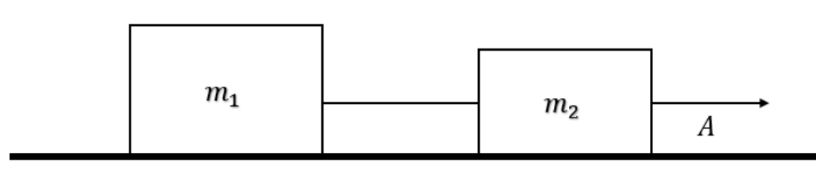
\includegraphics{Figura 1.png}
            \caption{\textcolor{white}{Sistema de dos bloques amarrados}}
            \label{fig 1}
        \end{figure}
    
    Resolución:\newline

    Tomando en cuenta el siguiente diagrama de cuerpo libre:

        \begin{figure}[h]
            \centering
            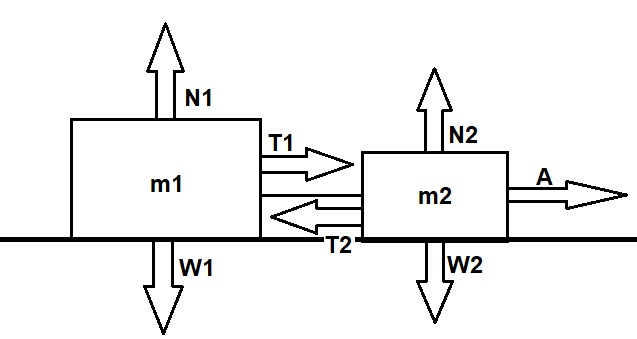
\includegraphics{DCL.jpg}
            \caption{\textcolor{white}{Diagrama cuerpo libre de dos bloques amarrados}}
            \label{Diagrama 1}
        \end{figure}

    Es fácil darse cuenta de que peso de las masas, en este caso, es paralelo a la fuerza normal, por lo que inmediatamente quedan descartadas ambas fuerzas a la hora de calcular la suma de las fuerzas que afectana a cada una de las masas, las cuales, por cierto, son:

        \begin{equation}
            \label{F's en m1}
            \sum 1=m_{1}\vec{a}\quad \Rightarrow \quad \vec{T_{1}}=m_{1}\vec{a}
        \end{equation}

        \begin{equation}
            \label{F's en m2}
            \sum 2=m_{2}\vec{a}\quad \Rightarrow \quad \vec{A}-\vec{T_{2}}=m_{2}\vec{a}
        \end{equation}

    De este modo, es factible decir que la suma de los lados derechos de \ref{F's en m1} y \ref{F's en m2} nos darán un despeje aceptable para la aceleración, tal que así:

        \begin{equation}
            \label{aceleración en sistema de cuerdas}
            \vec{T}_{1}+\vec{A}-\vec{T}_{2}=m_{1}\vec{a}+m_{2}\vec{a}\quad
            \Rightarrow \quad
            \textcolor{red}{\vec{a}=\frac{\vec{T_{1}}-\vec{2}+\vec{A}}{m_{1}+m_{2}}}
        \end{equation}
    
    Con lo cuál ya tendríamos una fórmula sencilla para la aceleración de todo el sistema en \ref{aceleración en sistema de cuerdas}.\newline

    Ahora, para la tensión en la cuerda, hay que destacar que en la imagen \ref{Diagrama 1} las fuerzas que actuan sobre la cuerda son, precisamente, la tensión 1 y la tensión 2, por lo cual la fórmula para la tensión sería:

        \begin{equation}
            \label{tensión en sistema de cuerdas}
            \vec{T}_{1}=m_{1}\vec{a},\quad
            \vec{T}_{2}=\vec{A}-m_{2}\vec{a}\quad
            \Rightarrow \quad
            \textcolor{red}{T=\vec{T}_{1}+\vec{T}_{2}=\vec{a}(m_{1}-m_{2})+\vec{A}}
        \end{equation}

    Y así se obtine la ecuación que determina la tensión de la cuerda, reflejada en \ref{tensión en sistema de cuerdas}.
    
\end{enumerate}
    
    \pagestyle{fancy}
            \fancyhf{}
            \rhead{\textcolor{white}{\thepage}}
            \cfoot{\textcolor{white}{Jordán Aarón Duarte Martínez}}
                 \lhead{\textcolor{white}{\textsc{Punto extra}}}

\section*{Punto extra}

Investiguen que hace la paquetería ``hyperref” y expliquen que hace, citen su fuente donde fue investigado.\newline

El paquete hyperref, por \cite{hyperref}, ($\backslash$usepackage$\{$hyperref$\}$) es usado para tener un control adecuado de todo tipo de links y referencias a lo largo del texto, siendo esto último gracias a que las referencias previas citadas por el comando $\backslash$ref$\{$$\}$ se convierten automáticamente en links (que al darles click te llevaran directo a dónde está el objeto al que se hace referencia) al momento de aplicar la paquetería en cuestión.\newline

Antes de continuar, cabe señalar que también nos da un mejor control en documento extensos al convertir en enlaces las líneas en la tabla de contenidos en cuestión.\newline

Esta paquetería nos da los siguientes comandos nuevos:

\begin{itemize}
    \item $\backslash$url$\{$link$\}$.\newline
    
    Este nos permite introducir cualquier link web en su forma  ``real" para hacerle referencia, y al clicar en él ir a la página de este.
    
    \item $\backslash$href$\{$link/nombre del archivo local$\}$$\{$nombre con el que aparecera en el texto$\}$\newline

    Sirve para lo mismo que el anterior comando, pero tiene la diferencia de que pone el enlace ``oculto" y muestra, en su lugar, una palabra o frase que le atribuyamos; además de que con éste también se puede hacer referencia a archivos locales del documento.
    
    \item $\backslash$hyperlink$\{$la palabra/oración$\}$$\{$nombre con el que aparecera en el texto$\}$\newline

    Sirve para ``enlazar" cualquier palabra del documento a otra parte usando como ``link de referencia" (resaltado de algún color) la palabra que elijamos.
    
    \item $\backslash$hypertarget$\{$la palabra/oración$\}$$\{$nombre con el que aparecera en el texto$\}$\newline

    En palabras simples, funciona para lo mismo que el anterios comando, pero tiene la diferencia de que no resalta el texto de ningún color.
    
\end{itemize}

Cabe añadir que esta paquetería nos da la opción de personalizar ciertos parametro que se muestran en la tabla \ref{tabl mods links} y la tabla \ref{tabl mods PDF}, siendo los de la primera tabla modificaciones para los links, y el segundo modificaciones especificas para agregar información adicional en el PDF, y cambiar la forma en que el visor del PDF muestra el archivo.\newline

NOTA: Para ingresar todas estas modificaciones es necesario usar el comando $\backslash$hypersetup$\{$opción1,opción2,...$\}$.

\begin{table}[h]
    \caption{\textcolor{white}{Modificaciones de links}}
    \label{tabl mods links}
    \centering
    \begin{tabular}{|l|l|l|}\hline
        \textcolor{white}{\textbf{Opción}} & \textcolor{white}{\textbf{Valor default}} & \textcolor{white}{\textbf{Descripción}}\\\hline
        \textcolor{white}{hyperindex} & \textcolor{white}{true} & \textcolor{white}{Núm.s de pág.s de las entradas del índice convertidas en hipervínculos}\\\hline
        \textcolor{white}{linktocpage} & \textcolor{white}{false} & \textcolor{white}{Hace que los números de página, y no el texto, se vinculen al índice}\\\hline
        \textcolor{white}{breaklinks} & \textcolor{white}{false} & \textcolor{white}{Permite que los enlaces se dividan en varias líneas}\\\hline
        \textcolor{white}{colorlinks} & \textcolor{white}{false} & \textcolor{white}{Colorea el texto de los enlaces y anclas (visibles en la versión impresa)}\\\hline
        \textcolor{white}{linkcolor} & \textcolor{white}{red} & \textcolor{white}{Colorea los enlaces internos normales}\\\hline
        \textcolor{white}{anchorcolor} & \textcolor{white}{black}	& \textcolor{white}{Color para el texto de anclaje}\\\hline
        \textcolor{white}{citecolor} & \textcolor{white}{green} & \textcolor{white}{Colorea las citas bibliográficas}\\\hline
        \textcolor{white}{filecolor} & \textcolor{white}{cyan} & \textcolor{white}{Colorea los enlaces que abren archivos locales}\\\hline
        \textcolor{white}{urlcolor} & \textcolor{white}{magenta} & \textcolor{white}{Color para las URL vinculadas}\\\hline
        \textcolor{white}{frenchlinks} & \textcolor{white}{false} & \textcolor{white}{Versalitas en lugar de colores para los enlaces}\\\hline
        \textcolor{white}{urlstyle$\{$same$\}$} & \textcolor{white}{same} & \textcolor{white}{Enlaces mostrados como texto normal}\\\hline
    \end{tabular}
\end{table}

\begin{table}[h]
    \caption{\textcolor{white}{Modificaciones del PDF}}
    \label{tabl mods PDF}
    \centering
    \begin{tabular}{|l|l|l|}\hline
        \textcolor{white}{\textbf{Opción}} & \textcolor{white}{\textbf{Valor default}} & \textcolor{white}{\textbf{Descripción}}\\\hline
        \textcolor{white}{bookmarks} & \textcolor{white}{true} & \textcolor{white}{Los marcadores de Acrobat están escritos de forma similar al índice}\\\hline
        \textcolor{white}{bookmarksopen} & \textcolor{white}{false} & \textcolor{white}{Marcadores motrados con todas sus subramificaciones expandidas}\\\hline
        \textcolor{white}{citebordercolor} & \textcolor{white}{0 1 0} & \textcolor{white}{Color del recuadro alrededor de las citas en formato RGB}\\\hline
        \textcolor{white}{filebordercolor} & \textcolor{white}{0 .5 .5} & \textcolor{white}{Color del recuadro alrededor de los links en formato RGB}\\\hline
        \textcolor{white}{linkbordercolor} & \textcolor{white}{1 0 0} & \textcolor{white}{Color del recuadro alrededor de los links normales en formato RGB}\\\hline
        \textcolor{white}{menubordercolor} & \textcolor{white}{1 0 0} & \textcolor{white}{Color del cuadro alrededor de los enlaces del menú en formato RGB}\\\hline
        \textcolor{white}{urlbordercolor} & \textcolor{white}{0 1 1} & \textcolor{white}{Color del cuadro alrededor de los enlaces a las URL en formato RGB}\\\hline
        \textcolor{white}{pdfpagemode} & \textcolor{white}{empty} & \textcolor{white}{Abre el PDF como: UseThumbs, UseOutlines o FullScreen}\\\hline
        \textcolor{white}{pdftitle} &  & \textcolor{white}{Establece el título del documento}\\\hline
        \textcolor{white}{pdfauthor} &  & \textcolor{white}{Establece el autor del documento}\\\hline
        \textcolor{white}{pdfstartpage} & \textcolor{white}{1} & \textcolor{white}{Determina en qué página se abre el archivo PDF}\\\hline
    \end{tabular}
\end{table}

\printbibliography

\end{document}